\chapter{Technical background}

\setcounter{section}{2}
\setcounter{subsection}{0}

\subsection{Single-page applications}

As previously described SPAs introduce new demands regarding architecture and structure on the client side. To understand how these problems can be approached it is important to understand the basics behind how a single-page application works. There is yet no formal definition that describes what a SPA is. Many developers have their own view of what it exactly means, but Ali Mesbah and Arie van Deursen \cite{spa_def} have stated a quite clear definition in their paper about SPAs:

\begin{quote}
"The single-page web interface is composed of individual components which can be updated/replaced independently, so that the entire page does not need to be reloaded on each user action."
\end{quote}

The definition includes a number of key attributes that help to define a SPA:

\begin{itemize}
	\item {\bf Web interface} - Used on the web, focuses on user interfaces.
	\item {\bf Individual components} - It's divided into smaller components that coop with each other.
	\item {\bf Updates and replaces} - A component can at any time be changed or replaced with another component.
	\item {\bf Reloading} - The entire page is never reloaded even though new content may be loaded into some sections.
	\item {\bf User actions} - The SPA is responsible for handling user actions such as input from mouse and keyboard.
\end{itemize}

When running a Javascript SPA the browser first makes a request to the web server. The web server will then respond with the Javascript client including the resources needed to run it. Once the client is transferred it will be initialized and it will be ready to be run. When the user interacts with the client, such as clicking on graphical elements, this may require new data to be fetched from the server. Instead of reloading the entire page the client will instead make a small request to the API on the web server. The API is simply an interface that allows the clients to communicate with the server in a data format that is easy to understand for both the client and server \cite{grb_wapi_rest}. A typical flow of communication for a SPA can be seen in figure \ref{fig:flow}.

\begin{figure}[h!]
	\centerline{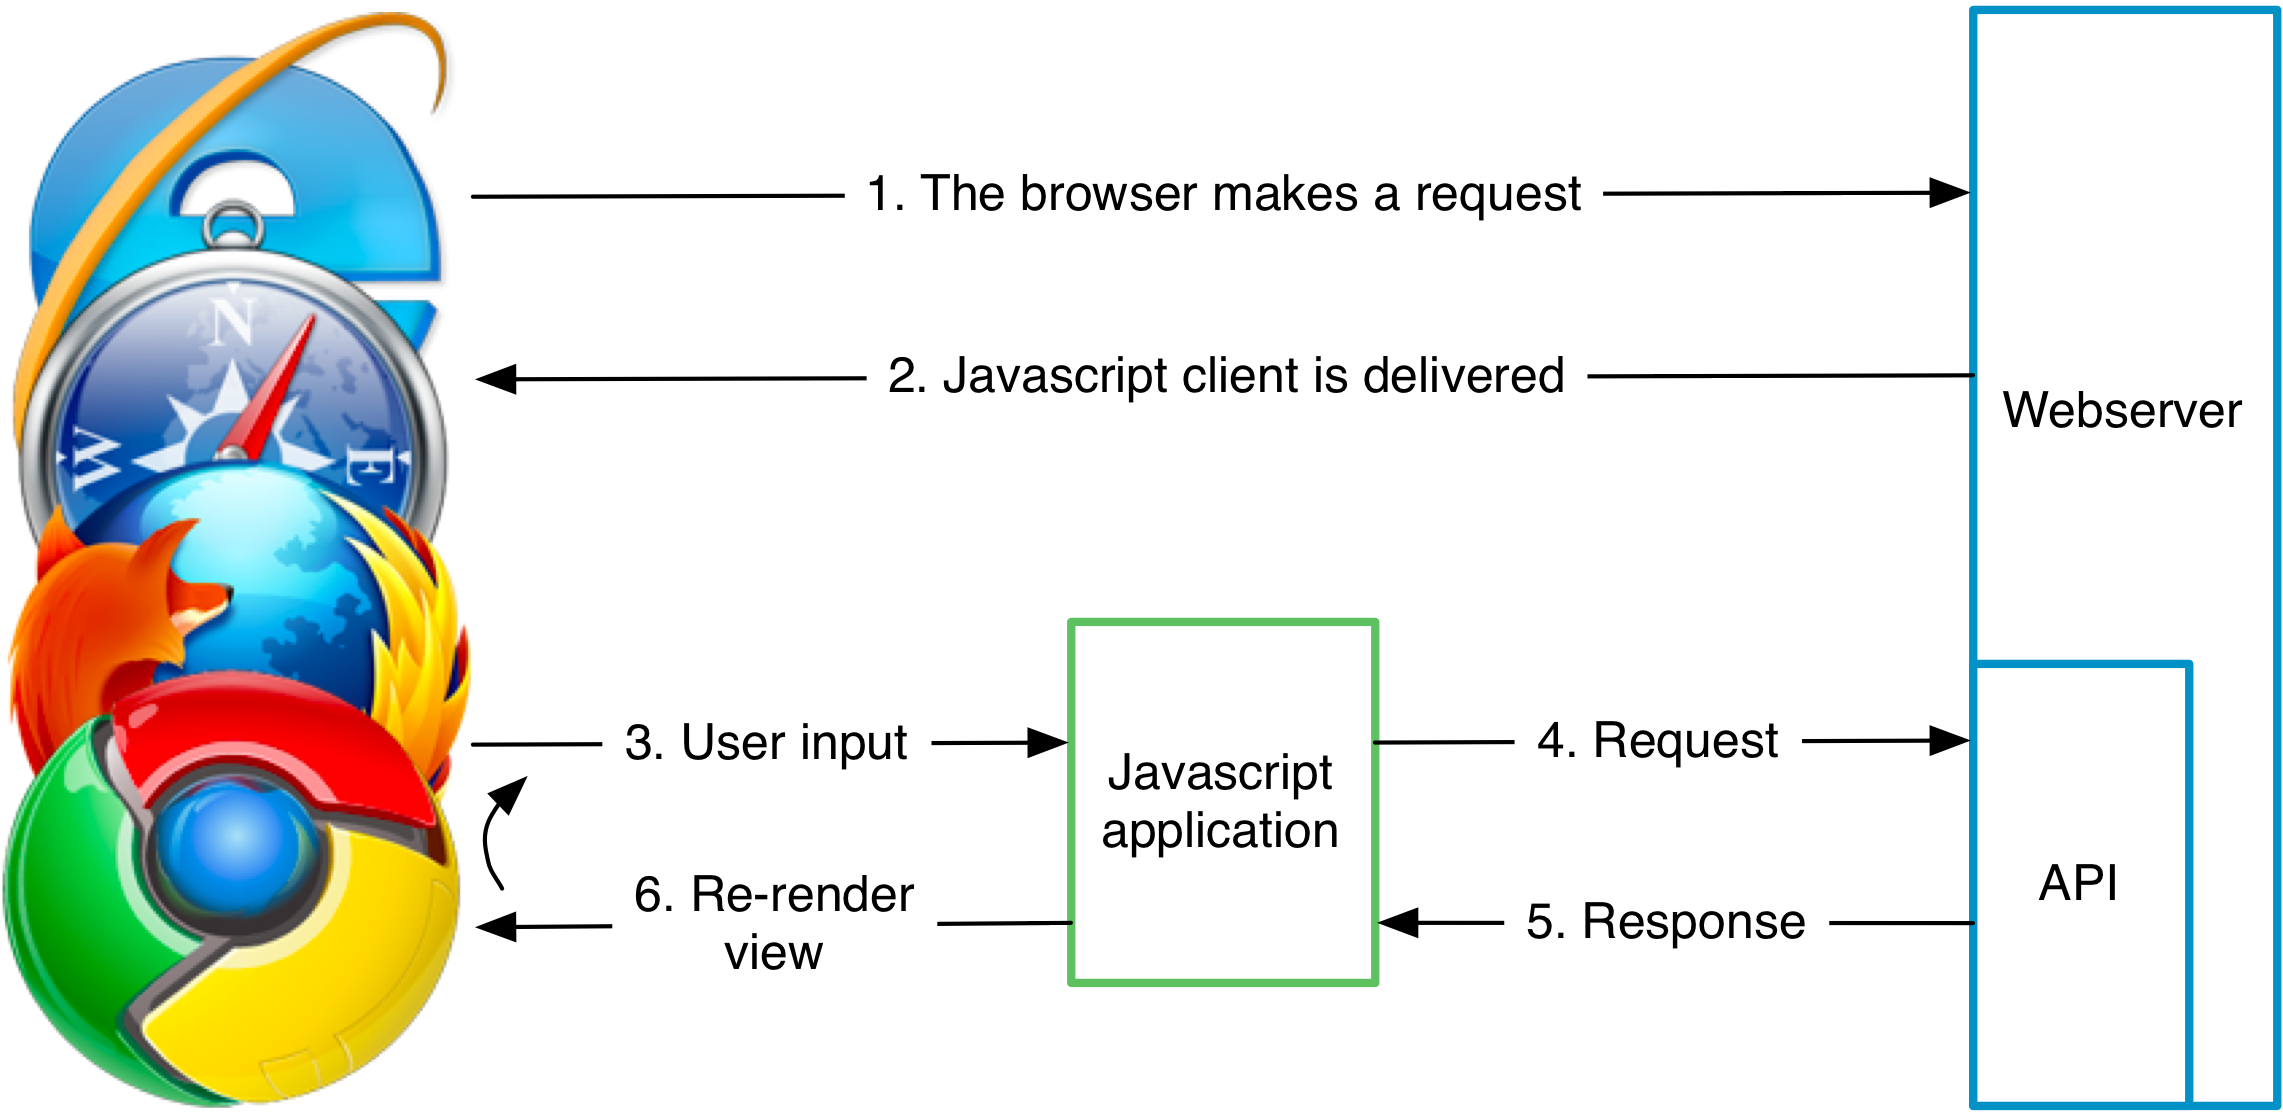
\includegraphics[width=150mm]{gfx/flow.png}}
	\caption{The flow of communication between a browser and the web server.}
	\label{fig:flow}
\end{figure}

\subsection{URLs, routes and states}
The URL structure of a website is an fundamental aspect to consider. In order to provide linkable and shareable URLs it is important that the URL is unique for the application's state. If the same URL would be used for several states they would not be accessible directly from the address bar, which would become impractical if a user stores or shares the current URL. The Javascript application needs to be able to map a URL into a certain state, this is often done by a routing component. It takes the URL that the user provides and decodes it into a state so that the correct components can be initialized and presented to the user. The routing component also needs to be able to update the URL if the application's state is changed. The HTML5 draft provides a history API to allow a Javascript client to change the URL during runtime without reloading the page \cite{w3c_history}. To support older browsers that do not support the history API the hashbang technique can instead be used \cite{html5_missing_manual}. The idea is to add {\em \#!/state} to the URL, the characters that comes after the hashmark (\#) will not be sent to the server and can instead be used by the Javascript client to detect a certain state of the application.

Both the HTML5 history API and the hashbang technique will keep the back-button behavior intact. When the user hits the back-button in the browser the URL will simply change to the last visited URL. The Javascript application will recognize a change of URL and will load the content once again. By having a system like this it becomes possible to use URLs just as if the pages were rendered by a backend system instead by a Javascript application.

\subsection{API communication}

In order for the client to dynamically fetch data from the server an API is needed in between. The API describes how data is being transferred, what data format is being used and what methods are available.

One of the most common ways of letting the client asynchronously communicate with the server is via AJAX (Asynchronous Javascript and XML). AJAX allows the client to asynchronously fetch and post data to the server after the page has been loaded. However, AJAX has no native support for letting the server push data to the client. The client must always initialize a new connection and then poll the server for new data \cite[p. 491]{js_def_guide}. To enable the server to push data to the client other techniques can instead be used, e.g. the websocket API in the HTML5 draft which supports bi-directional communication. This will ease the load of the server and allows a faster and more responsive system.

When using a HTTP-based data transportation some kind of architectural structure is needed. The architecture describes how messages are formed so that both parties understand each other, e.g. what methods that are available and how data is transferred. It also often includes additional information about how authentication is handled, as well as the flow of communication. Common architectural structures are REST and SOAP.

The data format of a message describes the syntactical form of the objects that are transferred. Since HTTP messages are based on ASCII-characters \cite{http_rfc_message_standard} it is also commonly used when describing data objects. Common data formats used today are JSON, XML and plain text \cite{grb_wapi_rest}. 

\subsection{Templates}

In order to separate the presentation layer from the business logic, templates are often used. A template engine compiles HTML from a description written in a template language together with a set of data, it's commonly used for rendering the views in a Javascript application. When the data is changed the view can simply be re-rendered so that the user sees the correct version of it. A template engine is however a quite complex system, to generate HTML from a description an interpretation of the template language is required. Since these interpretations are done during runtime the performance is a crucial aspect to consider. Some frameworks have their own template engines while others use generic libraries in order to support template rendering. 

\subsection{Data bindings}

Data bindings are used to bind a set of data to a corresponding view. One-way data bindings allow a view to be automatically re-rendered when its data is changed. Some frameworks, like Angular JS, support a two-way data bindings that also allow the data to be updated corresponding to changes in the view \cite{angularjs_twoway_databinding}. This is quite a powerful technique since all logic behind a view now is managed by the framework which makes it easier for the developer to get things working. Important to note is that no logic or complexity is removed, it is just moved to the framework. However, a framework must support a wide range of HTML-elements even though all of these are not used in the application. This often affects the performance of the application and two-way data bindings can sometimes become overkill, especially for smaller applications.

\subsection{Testing a Javascript application}

\label{sec:background_testing}

Testing comes in many forms and shapes during a project. During the development phase unit tests are commonly used to drive the development. It's used as a tool by the developers to ensure that all the functionality is kept intact. The use of a testdriven approach to develop software is becoming more and more popular \cite{tdd_popular}. However, developing Javascript applications with a testdriven approach can be tricky. The functionality behind a Javascript application tends to be tightly coupled with the user interface. This is simply the case since one of the most essential purposes of a Javascript applications is to interact with the user, which of course is done via the user interface. To write unit tests that interacts with the user interface is not trivial. It requires the unit test to trigger events on DOM-elements and then traverse the DOM and validate its content. If a view is even slightly changed this can break the test even if an acceptance test would still pass. Some architectures allow developers to instead write unit tests for what is underneath the graphical interface, making the tests easier to write and the result easier to validate. In the end unit testing will only ensure that the code is doing the right thing, not that the system is working as expected. High-level testing, such as acceptance testing, will always be needed to validate the functionality from a user perspective \cite{acceptance_testing}.

\subsection{Search engine optimization}

Search engine optimization is an important aspect of today's web services. Search engines such as Google, Bing and Yahoo indexes webpages every day to make it easier for users to find what they are looking for. In order to get a high page rank it is important that the search engines can index the content of the web service to understand what it is about.

The indexing is done by a crawler. The crawler downloads a snapshot of the webpage and analyzes the HTML to find keywords, links and more. Even though the crawler itself is quite a complex system the support for Javascript is limited. Google crawler won't run any Javascript at all \cite{google_crawler_nojs}, even though there are other reports stating that it actually can run a limited amount of Javascript \cite{google_crawler_some_js}. Nevertheless, the limited support is a major issue when building Javascript-based sites that are to be indexed by a crawler.

In terms of the crawlers from Google, Bing and Yahoo is this solved by translating the URLs for AJAX-based services, this allows the webserver to serve static HTML snapshots instead of dynamic Javascript versions. When the crawler visits a website that has an URL that contains a hashbang (\#!) the site will be treated as an AJAX-based site. All characters after the hashbang are then sent as the GET parameter $\_escaped\_fragment\_$ \cite{escaped_fragment}. The reason for this is due to the HTTP specification stating that characters after a hashmark should not be included in the request to the webserver \cite{no_url_sent}. The webserver can check if the GET parameter $\_escaped\_fragment\_$ is set, if so is the client probably a crawler and a static HTML version is to be served. Figure \ref{fig:crawler_flow} shows how a typical crawler treats AJAX-based websites.

\begin{figure}[h!]
	\centerline{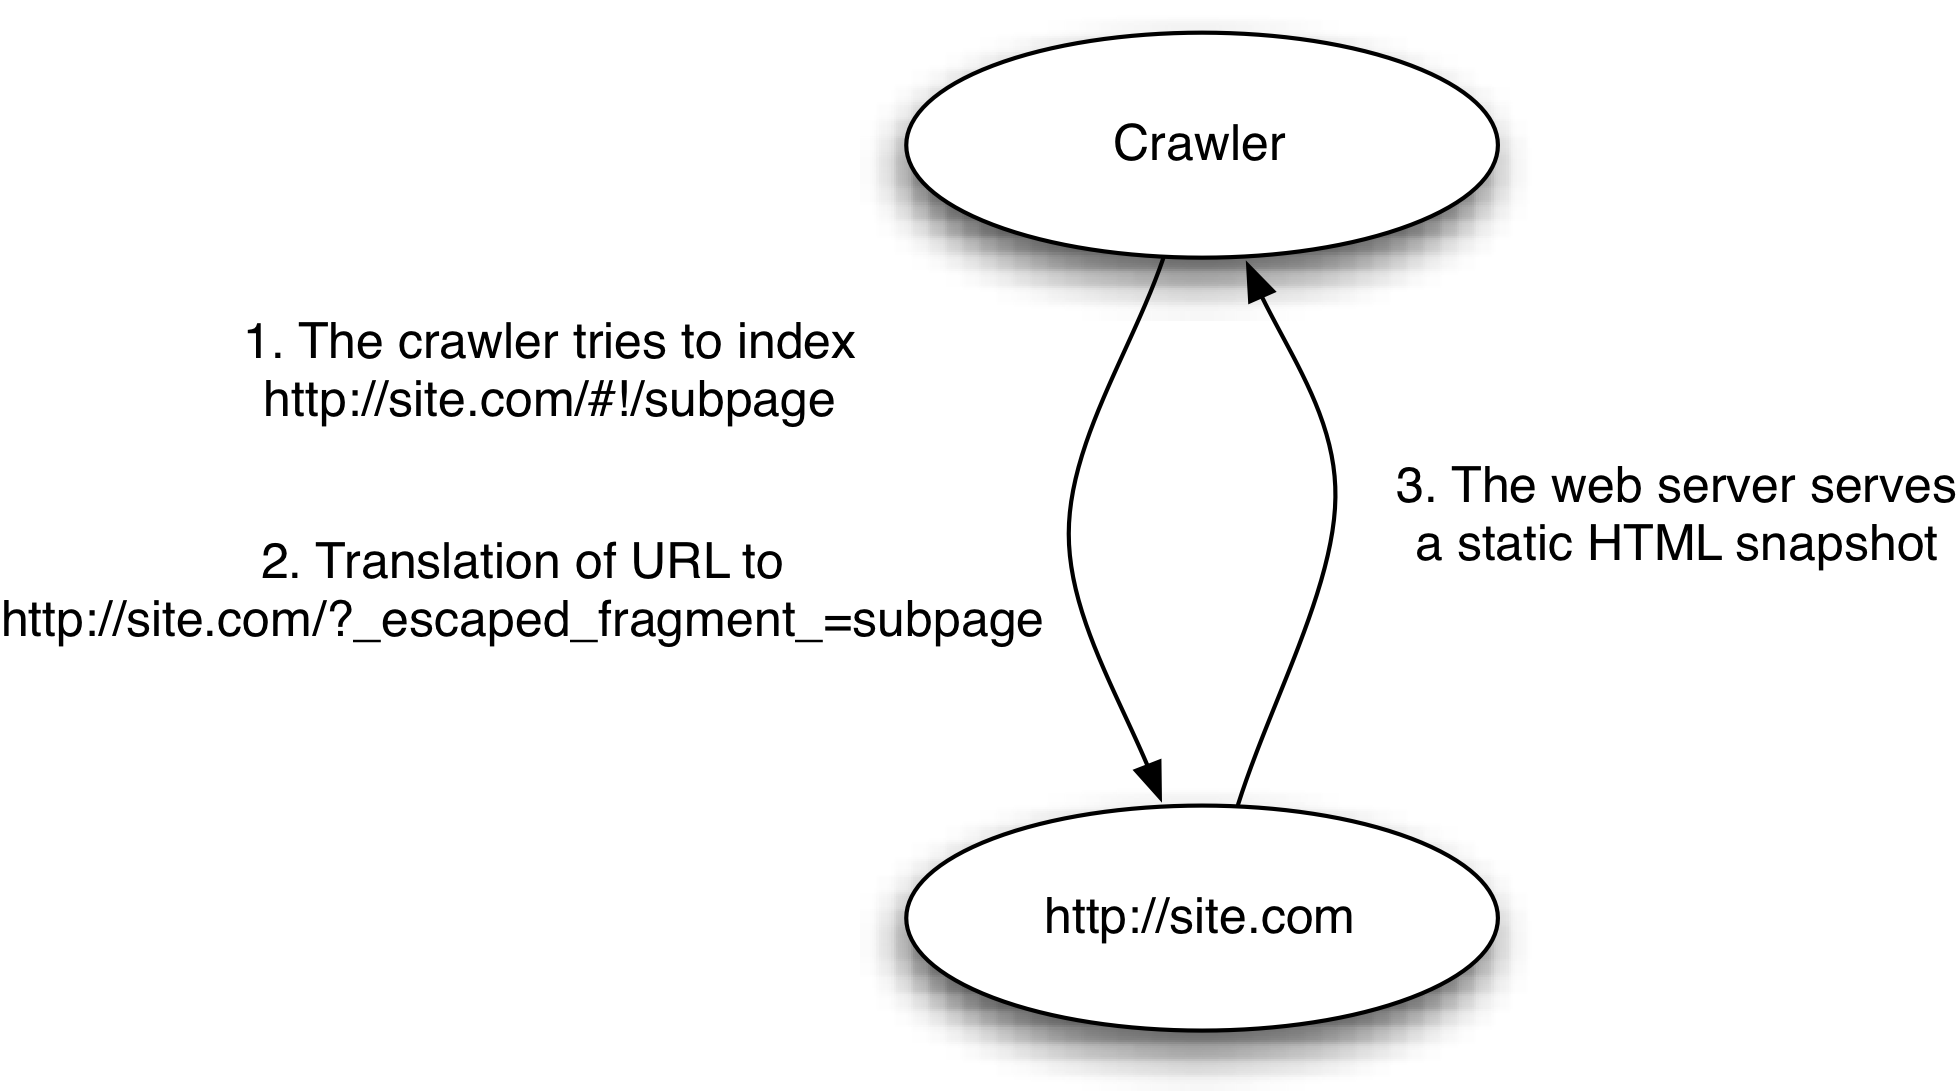
\includegraphics[width=120mm]{gfx/seo_flow.png}}
	\caption{The flow of how a typical crawler communicates with an AJAX-based website.}
	\label{fig:crawler_flow}
\end{figure}
